\chapter{Анализ трёх аспектов современных стран по Викиданным: возраст стран, популярные формы правления и этнохоронимы}
\label{ch:country}

Эта глава посвящена исследованию стран на основе базы знаний международного проекта Викиданные. С помощью SPARQL-запросов, вычисляемых на объектах типа ”страна” в Викиданных, получены: выведен список всех ныне существующих стран, перечень стран, упорядоченных по дате создания, список этнохоронимов стран, пузырьковая диаграмма с формами правления стран и граф соседних стран. Кроме того, сделаны отностительно полноты Викиданных по данной теме.
%%%%%%%%%%%%%%%%%%%%%%%%%%%%%%%%%%%%%%%%%%%%%%%%%%%%%%%
\section{Экземпляры}

%Используются следующие эксемпляры объекта <<Страна>>:
%\begin{itemize}
%	\item Объект: страна или \wdqName{country}{6256}, листинг~\ref{lst:country}
%	\item Свойство: экземпляр \href{https://www.wikidata.org/wiki/Property:P31}{instance of (P31)}.
%\end{itemize}

Построим список всех стран на английском и русском языках.

\begin{lstlisting}[ language=SPARQL, 
caption={\href{https://w.wiki/k6L}{Экземпляры объекта <<Страна>>}},
label=lst:country, 
escapebegin=ку,escapeend=ку-ку>
]
#List of countries in English and Russian
SELECT ?country ?label_en ?label_ru
WHERE
{
		?country wdt:P31 wd:Q6256. # country
		?country rdfs:label ?label_en filter (lang(?label_en) = "en").
		?country rdfs:label ?label_ru filter (lang(?label_ru) = "ru").
}
\end{lstlisting}

SPARQL-запрос (листинг ~\ref{lst:country}) имеет 205 записей на 2017 год и 175 записей на 2020 год.

Примерами наиболее полных и проработанных стран на Викиданных являются:  \wdqName{Соединённые Штаты Америки}{30}, \wdqName{Канада}{16}, \wdqName{Испания}{29}.

Почти пустыми и малоинформативными странами были: \wdqName{Сахарская Арабская Демократическая Республика}{40362}, \wdqName{Приднестровская Молдавская Республика}{907112}, \wdqName{Косово}{1246}.

%%%%%%%%%%%%%%%%%%%%%%%%%%%%%%%%%%%%%%%%%%%%%%%%%%%%%%%
\section{Возраст стран}

Построим список стран, отсортированных по дате основания страны (первом упоминании о стране).

%Используются:

%\begin{itemize}
%	\item Объект: страна или \wdqName{country}{6256}, листинг~\ref{lst:age_of_country}
%	\item Свойство: дата основания или \href{https://www.wikidata.org/wiki/Property:P571}{inception (P571)}.
%\end{itemize}

\begin{lstlisting}[ language=SPARQL, 
caption={\href{https://w.wiki/k6M}{Даты основания стран}},
label=lst:age_of_country, 
escapebegin=ку,escapeend=ку-ку>
]
SELECT ?country ?countryLabel ?inception
WHERE
{
		?country wdt:P31 wd:Q6256. # country
		?country wdt:P571 ?inception. # inception
		
		SERVICE wikibase:label { bd:serviceParam wikibase:language "en" }
}

ORDER BY (?inception)
}
\end{lstlisting}

SPARQL-запрос (листинг ~\ref{lst:age_of_country}) имеет 112 записей на 2017 год и 199 записей на 2020.

В результате выполнения запроса получен список стран с датами их создания. Например, \wdqName{Абхазия}{23334} - 1 января 0786, \wdqName{Россия}{159} - 1 января 0862, \wdqName{Косово}{1246} - 17 февряля 2008, \wdqName{Южный Судан}{958} - 9 июля 2011. Годы, в которые было создано наибольшее количество стран - 1991 (17 стран), 1812 (6 стран) и 1918 (5 стран).

Лидерами среди стран по количеству свойств в Викиданных, по версии ProWD, являются \wdqName{Израиль}{801} и \wdqName{Франция}{142} (по 127 свойств), наименьшее количество свойств у \wdqName{Демократической Республики Вьетнам}{172640} (24 свойства).

\subsection{Полнота Викиданных}

Проанализируем полноту Викиданных.

По данным <<Общероссийского классификатора стран мира>> на земле существует 251 страна.

В этой задаче не учитываются древние, уже не существующие государства (например: \wdqName{Ассирия}{41137}, поскольку они являются экземпляром не объекта <<country>>, а объекта <<former country>> (бывшие страны). Отметим, что количество бывших стран на порядок больше существующих ныне стран.

По данным категории <<Алфавитный список стран и территорий>> Русской Википедии существует 252 страны(В <<Общероссийском классификаторе стран мира>> недостает Косово).

По данным категории <<List of sovereign states>> Английской Википедии существует 206 стран.

Не всегда можно точно указать дату основания страны по разным причинам: отсутствие, недостаток или противоречие письменных источников. Например, основание Древнерусского государства связывают с призванием варяжского князя Рюрика в 862 году, но точной даты нет (объект \wdqName{Россия}{159}). Так же некоторым современным странам предшествовали ряд других и дату образования какого из них считать за дату создания современной страны ‒ это вопрос открытый (например, \wdqName{Монголия}{711}).

\subsection{Страны с незаполненной датой основания}

Выведем список стран с пустым свойством <<дата основания>>:

%Используются:

%\begin{itemize}
%	\item Объект: страна или \wdqName{country}{6256}, листинг~\ref{lst:without_inception}
%	\item Свойство: дата основания или \href{https://www.wikidata.org/wiki/Property:P571}{inception (P571)}.
%\end{itemize}

\begin{lstlisting}[ language=SPARQL, 
caption={\href{https://w.wiki/k6q}{Страны с незаполненной датой основания}},
label=lst:without_inception, 
escapebegin=ку,escapeend=ку-ку>
]
SELECT ?country ?countryLabel 
WHERE
{
		?country wdt:P31 wd:Q6256. # country
		
		MINUS { ?country wdt:P571 [] } . # inception of country is empty
		SERVICE wikibase:label { bd:serviceParam wikibase:language "en" }
}
}
\end{lstlisting}

SPARQL-запрос (листинг ~\ref{lst:without_inception}) имеет 100 записей на 2017 год и 7 записей на 2020 год.
%%%%%%%%%%%%%%%%%%%%%%%%%%%%%%%%%%%%%%%%%%%%%%%%%%%%%%%
\section{Этнохоронимы на русском языке}

Этнохороним — название жителей определённой местности, соотнесённое с топонимом. Например, Россия – россияне, россиянин, россиянка, Чехия – чехи, чех, чешка.

Помимо географического мотиватора, новых лексемы, используемые для определения происхождения либо принадлежности, происходят так же от этнических, политических, религиозных характеристик людей. 

Название жителей может исходить от наименования различных объектов земной поверхности — гор, островов, континентов. Так же обозначение места происхождения людей может зависеть от политико-административного делению. Например, для обозначения гражданства; Украина — украинцы, Канада - канадцы. Внутригосударственное деление так же может породить новые наименования, Крым — крымчане.

Построим список стран у которых есть этнохоронимы на русском языке.

Выведем список стран с пустым свойством <<дата основания>>:

%Используются:

%\begin{itemize}
%	\item Объект: страна или \wdqName{country}{6256}, листинг~\ref{lst:demonym}
%	\item Свойство: этнохороним или \href{https://www.wikidata.org/wiki/Property:P1549}{demonym (P1549)}.
%\end{itemize}

\begin{lstlisting}[ language=SPARQL, 
caption={\href{https://w.wiki/k72}{Этнохоронимы на русском языке}},
label=lst:demonym, 
escapebegin=ку,escapeend=ку-ку>
]
SELECT ?country ?countryLabel 
WHERE
{
		?country wdt:P31 wd:Q6256.       # country
		?country wdt:P1549 ?demonym .    # demonym
		FILTER((LANG(?demonym)) = "ru")
		SERVICE wikibase:label { bd:serviceParam wikibase:language "ru" }
}

GROUP BY ?country ?countryLabel
\end{lstlisting}

SPARQL-запрос (листинг ~\ref{lst:demonym}) имеет 28 записей на 2017 год и 99 записей на 2020 год.

\subsection{Cписок этнохоронимов}

Выведем список всех этнохоронимом на русском языке.

\begin{lstlisting}[ language=SPARQL, 
caption={\href{https://w.wiki/k7A}{Cписок этнохоронимов}},
label=lst:list_demonym, 
escapebegin=ку,escapeend=ку-ку>
]
SELECT ?country ?countryLabel ?demonym
WHERE
{
		?country wdt:P31 wd:Q6256.      # country
		?country wdt:P1549 ?demonym .   # demonym
		FILTER((LANG(?demonym)) = "ru")
		SERVICE wikibase:label { bd:serviceParam wikibase:language "ru" }
}
\end{lstlisting}

SPARQL-запрос  (листинг ~\ref{lst:list_demonym}) имеет 83 записи на 2017 год и 222 записи на 2020 год.

\subsection{Страны с незаполненными этнохоронимами}

Построим список стран, у которых нет этнохоронимов на русском языке.

\begin{lstlisting}[ language=SPARQL, 
caption={\href{https://w.wiki/k7E}{Страны с незаполненными этнохоронимами }},
label=lst:without_demonym, 
escapebegin=ку,escapeend=ку-ку>
]
SELECT ?country ?countryLabel 
WHERE
{
		?country wdt:P31 wd:Q6256.              # country
		MINUS { ?country wdt:P1549 ?demonym.    # except with demonyms
			FILTER((LANG(?demonym)) = "ru") # in Russian
		}    

		SERVICE wikibase:label { bd:serviceParam wikibase:language "ru" }
}
GROUP BY ?country ?countryLabel
\end{lstlisting}

SPARQL-запрос  (листинг ~\ref{lst:without_demonym}) имеет 170 записей на 2017 год и 83 записи на 2020 год.

\subsection{Количество заполненных этнохоронимов у стран}

Выведем список стран, упорядоченный по количеству заполненных в Викиданных этнохоронимов.

\begin{lstlisting}[ language=SPARQL, 
caption={\href{https://w.wiki/k7K}{Количество заполненных этнохоронимов у стран}},
label=lst:count_demonym, 
escapebegin=ку,escapeend=ку-ку>
]
SELECT  ?country ?countryLabel (count(*) as ?count)
WHERE
{
		?country wdt:P31 wd:Q6256.      # country
		?country wdt:P1549 ?demonym .   # demonym
		SERVICE wikibase:label { bd:serviceParam wikibase:language "ru" }
}
GROUP BY ?country ?countryLabel 
ORDER BY DESC(?count)
\end{lstlisting}

SPARQL-запрос (листинг ~\ref{lst:count_demonym}) имеет 199 записей на 2017 год и 167 записей на 2020 год.

По данным на 2017 год наибольшее число этнохоронимов у Соединённых Штатов Америки (41 этнохороним), затем идут Великобритания (40), Германия (40) и Канада (36). А на 2020 год наибольшее число этнохоронимов у Германии (64 этнохоронима), Канады (60), США (60) и Польши (54).
%%%%%%%%%%%%%%%%%%%%%%%%%%%%%%%%%%%%%%%%%%%%%%%%%%%%%%%
\section{Формы правления стран}

Построим пузырьковую диаграмму форм правления стран.

%Используются:
%\begin{itemize}
%	\item Объект: страна или \wdqName{country}{6256}, листинг~\ref{lst:form_of_government}
%	\item Свойство: форма правления или \href{https://www.wikidata.org/wiki/Property:P122}{subject's government (P122)}.
%\end{itemize}

\begin{lstlisting}[ language=SPARQL, 
caption={\href{https://w.wiki/k7M}{Формы правления стран}},
label=lst:form_of_government, 
escapebegin=ку,escapeend=ку-ку>
]
SELECT ?bfog ?form (count(*) as ?count)
WHERE 
{
	?country wdt:P31 wd:Q6256. # country
	?country wdt:P122 ?bfog. # subject's government
	OPTIONAL {
		?bfog rdfs:label ?form
		filter (lang(?form) = "ru")
	}
}
GROUP BY ?bfog ?form
ORDER BY DESC(?count) ASC(?form)
\end{lstlisting}

В итоге получим SPARQL-запрос (листинг ~\ref{lst:form_of_government}), который имеет 30 записей на 2017 год и 29 записей на 2020 год.

В результате выполнения запроса мы получаем пузырьковую диаграмму с наиболее распространенными формами правления в странах по 2017 году на рис. ~\ref{fig:bubble_chart_forms_of_government_countries_2017}, по 2020 году на рис.~\ref{fig:bubble_chart_forms_of_government_countries_2020}.

\begin{figure}
	{
		\setlength{\fboxsep}{0pt}%
		\setlength{\fboxrule}{1pt}%
		\fcolorbox{gray}{gray}{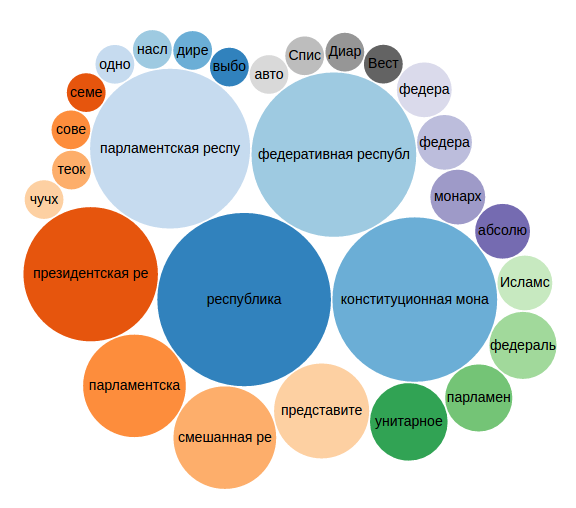
\includegraphics[width=\linewidth]{./chapter/country/Bubble_chart_forms_of_government_countries_according_to_Wikidata.png}}%
	}
	\caption{Пузырьковая диаграмма форм правления стран, 2017.
		\\			
		По данным на 2017 год основные формы правления стран: республика (в 20 странах), конституционная монархия (в 18 странах), федеративная республика (в 18 странах), парламентская республика (в 17 странах) и президентская республика (в 12 странах).}%
	\label{fig:bubble_chart_forms_of_government_countries_2017}%
\end{figure}

\begin{figure}
	{
		\setlength{\fboxsep}{0pt}%
		\setlength{\fboxrule}{1pt}%
		\fcolorbox{gray}{gray}{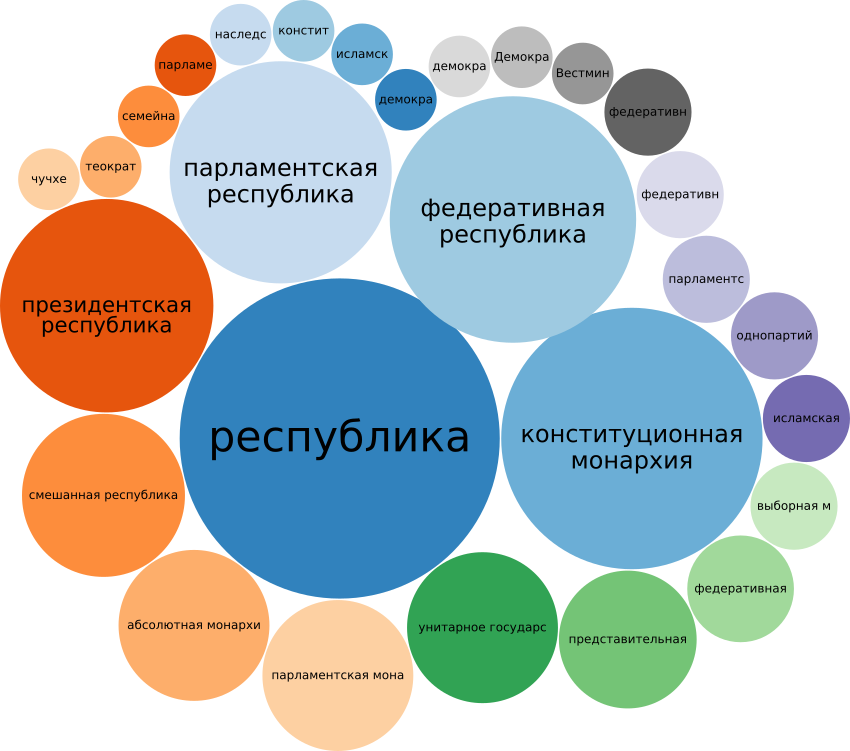
\includegraphics[width=\linewidth]{./chapter/country/Bubble_chart_forms_of_government_countries_according_to_Wikidata_2020.png}}%
	}
	\caption{Пузырьковая диаграмма форм правления стран, 2020.
	\\
	По данным на 2020 год  основные формы правления стран: республика (в 27 странах), конституционная монархия (в 18 странах), федеративная республика (в 16 странах), парламентская республика (в 13 странах) и президентская республика (в 12 странах).
}%
	\label{fig:bubble_chart_forms_of_government_countries_2020}%
\end{figure}

%%%%%%%%%%%%%%%%%%%%%%%%%%%%%%%%%%%%%%%%%%%%%%%%%%%%%%%
\section{Соседние страны}

Построим граф соседних стран.

%Используются:
%\begin{itemize}
%	\item Объект: страна или \wdqName{country}{6256}, листинг~\ref{lst:neighboring_countries}
%	\item Свойство: имеет границы с  или \href{https://www.wikidata.org/wiki/Property:P47}{shares border with (P47)}.
%\end{itemize}

\begin{lstlisting}[ language=SPARQL, 
caption={\href{https://w.wiki/k7P}{Соседние страны}},
label=lst:neighboring_countries, 
escapebegin=ку,escapeend=ку-ку>
]
SELECT ?country ?countryLabel ?sharesBorderWith ?sharesBorderWithLabel
WHERE
{
		?country wdt:P31 wd:Q6256.	# country
		SERVICE wikibase:label { bd:serviceParam wikibase:language "ru" }
		OPTIONAL { ?country wdt:P47 ?sharesBorderWith . }
}
\end{lstlisting}

SPARQL-запрос (листинг ~\ref{lst:neighboring_countries}) имеет 787 записей на 2017 год (рис. ~\ref{fig:neighboring_countries_2017}) и 698 записей на 2020 год (рис. ~\ref{fig:neighboring_countries_2020}).

\begin{figure}
	{
		\setlength{\fboxsep}{0pt}%
		\setlength{\fboxrule}{1pt}%
		\fcolorbox{gray}{gray}{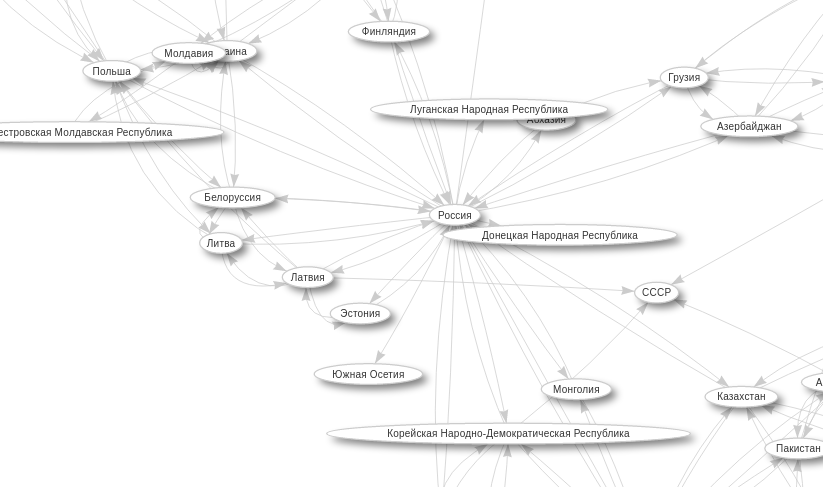
\includegraphics[width=\linewidth]{./chapter/country/Neighboring_countries_graph_in_russian_according_to_Wikidata_2017.png}}%
	}
	\caption{Граф соседних стран, в центре Россия, 2017.
	}%
	\label{fig:neighboring_countries_2017}%
\end{figure}

\begin{figure}
	{
		\setlength{\fboxsep}{0pt}%
		\setlength{\fboxrule}{1pt}%
		\fcolorbox{gray}{gray}{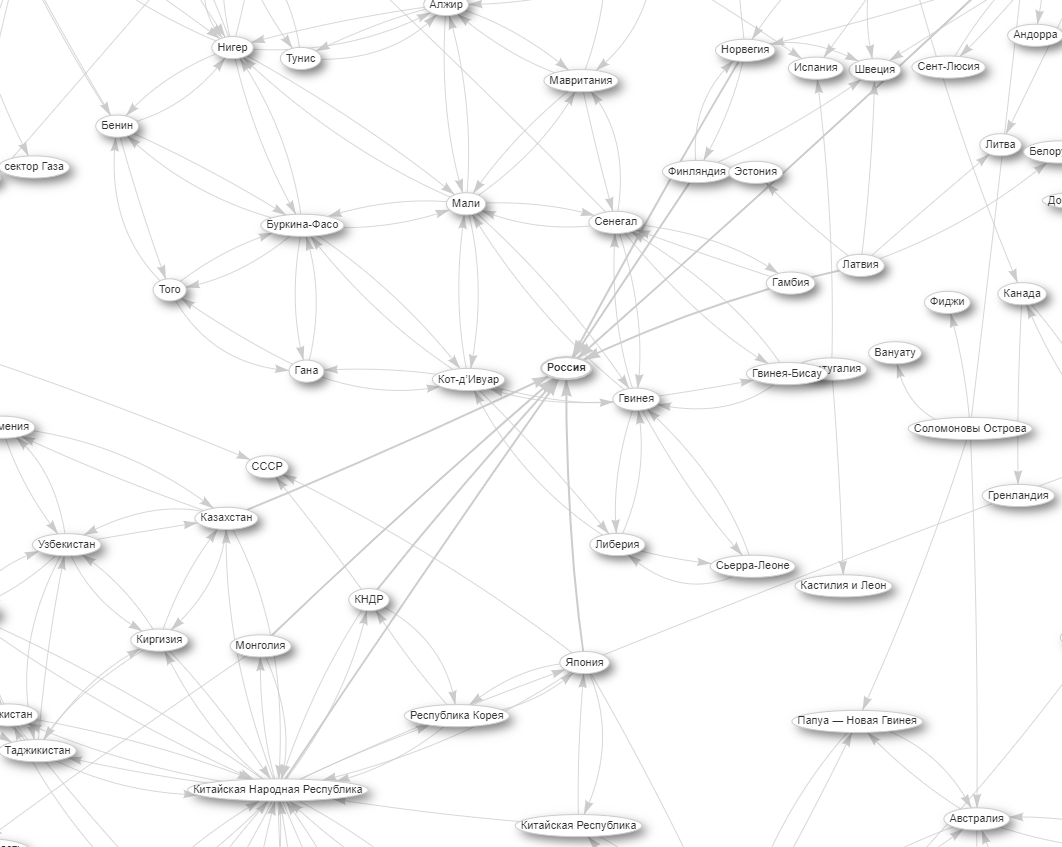
\includegraphics[width=\linewidth]{./chapter/country/Neighboring_countries_graph_in_russian_according_to_Wikidata_2020.png}}%
	}
	\caption{Граф соседних стран, в центре Россия, 2020.
	}%
	\label{fig:neighboring_countries_2020}%
\end{figure}

В результате выполнения запроса мы получаем граф с 787 ребрами на 2017 год (рис. ~\ref{fig:neighboring_countries_2017}) и 698 ребрами на 2020 год (рис. ~\ref{fig:neighboring_countries_2020}), где ребро – это соседство между двумя странами. Граф представляет из себя несколько связных компонент, так как есть островные страны, у которых нет соседей (например, Маврикий, Мальдивы, Мадагаскар).

%%%%%%%%%%%%%%%%%%%%%%%%%%%%%%%%%%%%%%%%%%%%%%%%%%%%%%%
\section{Упражнения}

\begin{enumerate}
	\item Для каждой страны выведите на экран список, включающий флаг и девиз страны.
	\item Выведите карту с отмеченными на ней столицами всех ныне существующих стран.
	\item В каждой части света вычислите первые пять стран с наибольшей плотностью населения.
	\item Построить столбчатую диаграмму демонстрирующую распределение количества стран по формам правления. Оцените, является ли это распределение тяжелым хвостом.
	\item Вывести список стран упорядоченных по числу соседей. У каких стран максимальное и минимальное количество соседей, какое среднее число соседей? Есть ли корреляция между этим показателем и каким-либо другим параметром стран?
\end{enumerate}